%% Basierend auf einer TeXnicCenter-Vorlage von Tino Weinkauf.

\documentclass[a4paper,oneside,10pt]{report}

\usepackage{listings}
\usepackage{color}

\definecolor{dkgreen}{rgb}{0,0.6,0}
\definecolor{gray}{rgb}{0.5,0.5,0.5}
\definecolor{mauve}{rgb}{0.58,0,0.82}

\lstset{frame=tb,
  language=Java,
  aboveskip=3mm,
  belowskip=3mm,
  showstringspaces=false,
  columns=flexible,
  basicstyle={\small\ttfamily},
  numbers=none,
  numberstyle=\tiny\color{gray},
  keywordstyle=\color{blue},
  commentstyle=\color{dkgreen},
  stringstyle=\color{mauve},
  breaklines=true,
  breakatwhitespace=true,
  tabsize=3
}


\usepackage[ngerman]{babel}
\usepackage[T1]{fontenc}
\usepackage[ansinew]{inputenc}
\usepackage[hidelinks]{hyperref}
\hypersetup{
	colorlinks=false,
	allcolors=black
}

\usepackage{lmodern} 

%\usepackage[backend=biber]{biblatex}

%\addbibresource{literatur.bib}

\usepackage{graphicx}

\graphicspath{{images/}}    % Bilderverzeichnis


%% Packages f�r Formeln %%%%%%%%%%%%%%%%%%%%%%%%%%%%%%%%%%%%%
%\usepackage{amsmath}
%\usepackage{amsthm}
%\usepackage{amsfonts}



\begin{document}

\pagestyle{empty} 

\title{Entwicklung eines Remote Method Invocation Systems}
\author{Emil Watz}
\maketitle

\tableofcontents 
\cleardoublepage 

\pagestyle{plain} 



\chapter{Anforderungen an das System}

\section{Verbindung des Server-Objekts mit dem Client-Objekt}

Es k�nnen mehrere Server-Objekte erstellt werden, deren Funktionen �ber das Netzwerk aufrufbar sind. Der Client kann sich mit einem der Server-Objekte verbinden. Es muss daher ein Mechanismus entwickelt werden, der die Auswahl eines Server-Objekts erm�glicht. Diese Auswahl geschieht �ber einen Namensdienst (siehe \ref{anf_namensdienst}).

\section{Entferntes Aufrufen}

Ein Client soll Funktionen am Server aufrufen k�nnen, dieser Funktionsaufruf soll sich aber gleich Verhalten, wie ein lokaler Aufruf. Der R�ckgabewert muss also vom Server zur�ck an den Client gesendet werden. Es k�nnen auch Parameter vom Client an den Server mitgegeben werden. Es muss auch eine L�sung f�r Exceptions geben. 
Au�erdem muss ein Verhalten f�r den Verbindungsabbruch definiert werden. Weiters muss auch beachtet werden, dass Funktionen �berladen werden k�nnen. 

\subsection{Benutzerdefinierte Typen}

Es k�nnen auch, sofern m�glich, benutzerdefinierte Typen als R�ckgabe- und Parameter verwendet werden, sowohl der Server, als auch der Client m�ssen nat�rlich �ber diesen Typen verf�gen. Hierbei muss wieder eine Fehlerbehandlung erfolgen. Die Definition von benutzerdefinierten Typen muss als Protocol Buffer erfolgen!

\section{gRPC-Einsatz}

Zus�tzlich zu dem RMI-System soll auch noch gRPC eingesetzt werden. Dieser Einsatz wird im Rahmen eines Namensdienstes implementiert. Mit dem Service k�nnen Server-Objekte unter einem bestimmten Namen angemeldet werden. Clients k�nnen dann �ber den Namen bestimmte Objekte ansprechen und deren Funktionen aufrufen. 

\section{Optionale Anforderungen}

Eine optionale Anforderung an das System, welche die Bedienung wesentlich erleichtern w�rde, ist die (teilweise) automatische Generierung des Client-Stubs und des Server-Skeletons. 

\chapter{Umsetzung}

\section{Klassendiagram}

\begin{figure}[h]
\centering
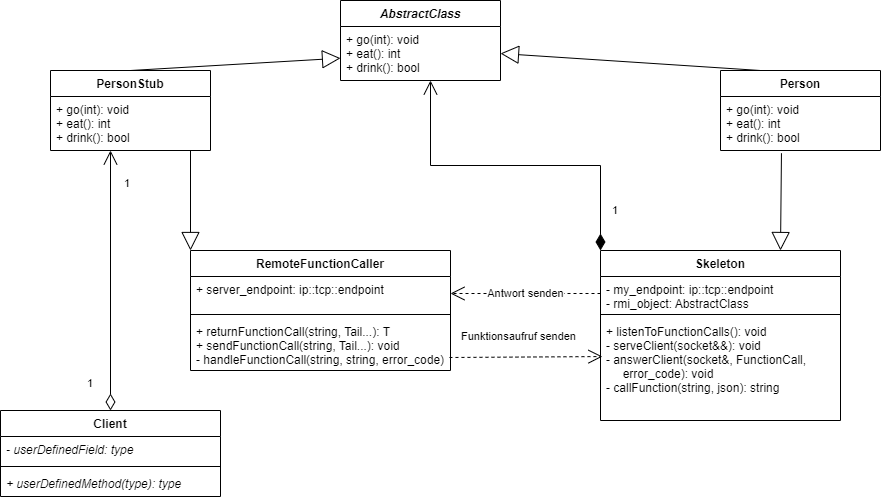
\includegraphics[width=12cm]{class_diagram}
\caption[My Caption]{Klassendiagram des RMI Systems}
\end{figure} 

\subsection{Abstrakte Klasse (AbstractClass)}

Die meisten Remote Method Invocation Systeme verwenden ein Interface, um die Methoden zu definieren. Da es in C++ keine Interfaces gibt, wird daher eine abstrakte Klasse verwendet, welche eine Anzahl an virtuellen ("`virtual"') Funktionen deklariert.

Diese Methodendeklaration m�ssen vor der Benutzung vom User erstellt werden. Im Klassendiagramm werden die Beispielfunktionen "`method1"', "`method2"' verwendet

\subsection{Client Stub}

Die \emph{Client Stub}-Klasse erbt von der abstrakten Klasse. Die Implementierungen der virtuellen Funktionen, senden einen Funktionsaufruf an die Skeleton-Klasse des Servers. Den R�ckgabewert oder die Exception erh�lt der Client Stub in serialisierter Form wieder vom Skeleton am Server. 

\subsection{Remote Object}

Das Remote Object enth�lt ein Template f�r die Funktion "`sendFunctionCall"', welches die Parameter in einen Protokoll Buffer umwandelt und an den Naming-Service sendet. 

\subsection{Skeleton-Klasse am Server}

Die Skeleton-Klasse am Server implementiert die benutzerdefinierte abstrakte Klasse. Die Implementierungen der virtuellen Funktionen wandeln die "`Funktionsaufruf-Nachrichten"', die vom Client Stub gesendet werden, in "`echte"' Funktionsaufrufe der Serverklasse um. Die R�ckgabewerte und Exceptions, welche die Funktionen der Serverklasse zur�ck

\subsection{Serverklasse}

Auch die Serverklasse implementiert die abstrakte Klasse. Die Implementierung der virtuellen Funktionen enth�lt in dieser Klasse die wirkliche Funktionslogik. 

\subsection{Client}

Der Client ist eine Klasse die komplett vom Benutzer konfiguriert werden kann. Zur Verwendung des Remote Method Invocation System ben�tigt er eine Instanz des Client Stubs. 

\subsection{Naming-Service} Der Naming-Service speichert alle Namen der Objekte, die bei dem Service registriert wurden. Er basiert auf gRPC und erweitert dadurch eine gRPC-Klasse. Objekte k�nnen mit einem Namen registriert werden, unter dem sie Funktionen bereitstellen k�nnen. 

\addtocontents{toc}{\protect\vspace*{\baselineskip}}

%% Literaturverzeichnis
%% ==> Eine Datei 'literatur.bib' wird hierf�r ben�tigt.
%% ==> Sie m�ssen hierf�r BibTeX verwenden (Projekt | Eigenschaften... | BibTeX)
%\addcontentsline{toc}{chapter}{Literaturverzeichnis}
%\nocite{*} %Auch nicht-zitierte BibTeX-Eintr�ge werden angezeigt.
%\bibliographystyle{alpha} %Art der Ausgabe: plain / apalike / amsalpha / ...
%\bibliography{literatur} %Eine Datei 'literatur.bib' wird hierf�r ben�tigt.

%% Abbildungsverzeichnis
%%\clearpage
%%\addcontentsline{toc}{chapter}{Abbildungsverzeichnis}
%%\listoffigures

%% Tabellenverzeichnis
%%\clearpage
%%\addcontentsline{toc}{chapter}{Tabellenverzeichnis}
%%\listoftables


%%%%%%%%%%%%%%%%%%%%%%%%%%%%%%%%%%%%%%%%%%%%%%%%%%%%%%%%%%%%%
%% ANH�NGE
%%%%%%%%%%%%%%%%%%%%%%%%%%%%%%%%%%%%%%%%%%%%%%%%%%%%%%%%%%%%%
%%\appendix
%% ==> Schreiben Sie hier Ihren Text oder f�gen Sie externe Dateien ein.

%\input{Dateiname} %Eine Datei 'Dateiname.tex' wird hierf�r ben�tigt.


\end{document}